\section{Experimentación y análisis}

\subsection{De Nueva York a Oxford}

Dado que existe un paralelísmo geográfico que acompaña a nuestro análisis, decidimos buscar algo para ejemplificarlo de manera visual. Elegimos la herramienta \textit{IP Fingerprints}\footnote{http://www.ipfingerprints.com/} que nos permite graficar, de forma aproximada, la ubicación de las máquinas por las que se pasa en la ruta, dándonos además, sus coordenadas; y con ellas, la posibilidad de ver en el mapa a dónde corresponden las mismas.\\
\\
\indent Sabemos que de \textit{Nueva York} a \textit{Oxford} hay un cambio de continente en el medio, y eso equivale a \textit{al menos un pasaje por un enlace submarino}. Como vista general, la ruta aproximada es la siguiente:
\begin{center}
	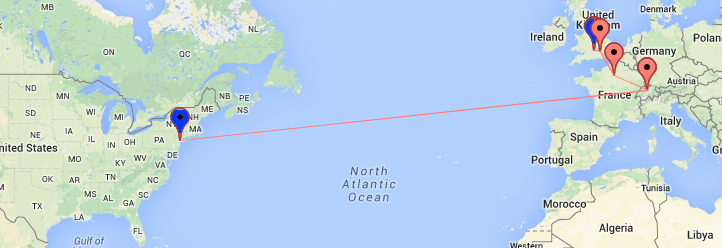
\includegraphics[scale=0.6]{graphics/new_york-oxford.png}
\end{center}

Tal y como lo sospechábamos, podemos observar \textit{enlaces internos en Estados Unidos} y \textit{enlaces internos en Europa}, unidos por un gran \textit{enlace submarino} entre ambos continentes. Decidimos distinguir los nodos de comienzo (en Nueva York) y fin de la ruta (en Oxford) pintándolos de color azul.\\
\\
\indent Viendo un poco más en detalle dentro de Nueva York, esta herramienta nos permitió ver que el primer hop es dentro de la ciudad de Nueva York, como vemos en esta imagen aumentada de la zona:

\begin{center}
	
\includegraphics[scale=0.6]{graphics/new_york_zoom.png}
\end{center}

Una vez que sale de ahí, viaja por enlace submarino a Europa. Más precisamente, a Suiza, como se ve en la siguiente imagen aumentada de la zona:

\begin{center}
	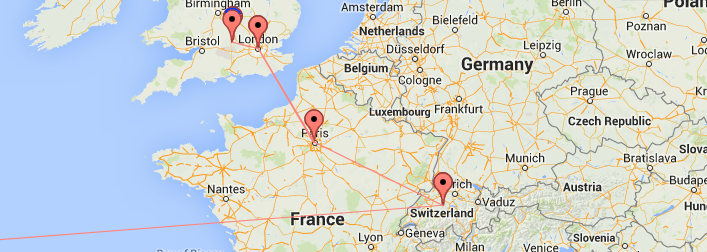
\includegraphics[scale=0.6]{graphics/europe_zoom.png}
\end{center}

Ahí envía paquetes en el mismo país unas 4 veces, hasta que sale y va a Francia, donde se envían 2 paquetes dentro de ese mismo país. Finalmente, de ahí pasa a la isla del Reino Unido, como vemos en la siguiente imagen:

\begin{center}
	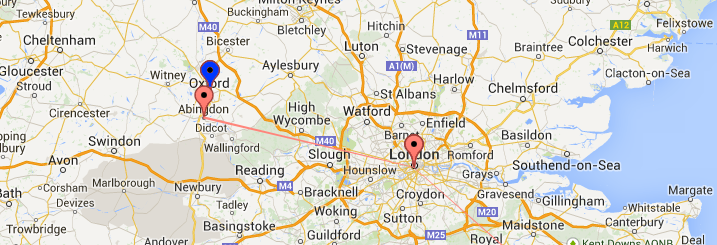
\includegraphics[scale=0.6]{graphics/united_kingdom_zoom.png}
\end{center}

Llega a Lóndres, envía 4 paquetes dentro de la ciudad, para luego ir a la ciudad donde finaliza el camino: Oxford. Ahí llega a la Universidad de Oxford, que es nuestro objetivo, salta a través de 3 máquinas, hasta efectivamente llegar a la que hostea el sitio web de la universidad.

\clearpage

\subsection{De Nueva York a Tokyo}

Empezaremos este análisis revisando la fórmula para \textit{$ZRTT_i$}.

$$ ZRTT_i = \frac{RTT_i - \overline{RTT}}{SRTT} $$

Lo que vemos es que el \textit{z score} de un hop corresponde a la comparación (diferencia) entre su \textit{$RTT_i$} y el RTT promedio, ponderado por el desvío estándar.

Para entender un poco mejor el \textit{z score} veamos qué significa que éste valga 0

\begin{equation}
	\frac{RTT_i - \overline{RTT}}{SRTT} = 0
\end{equation}
\\
\begin{equation}
	\frac{RTT_i}{SRTT} - \frac{\overline{RTT}}{SRTT} = 0
\end{equation}
\\
\begin{equation}
	RTT_i - \overline{RTT} = 0
\end{equation}
\\
\begin{equation}
	RTT_i = \overline{RTT}
\end{equation}

Sabiendo esto, podemos deducir cómo será el \textit{z score} cuando el \textit{$RTT_i$} es mayor al promedio

\begin{equation}
	RTT_i \geq \overline{RTT}
\end{equation}
\\
\begin{equation}
	RTT_i - \overline{RTT} \geq 0
\end{equation}
\\
\begin{equation}
	\frac{RTT_i}{SRTT} - \frac{\overline{RTT}}{SRTT} \geq 0
\end{equation}
\\
\begin{equation}
	\frac{RTT_i - \overline{RTT}}{SRTT} \geq 0
\end{equation}
\\
\begin{equation}
	ZRTT_i \geq 0
\end{equation}

Esto refuerza la intuición de que un RTT mayor al promedio significa un \textit{z score} mayor. Lo que queremos verificar es que a partir de cierto valor de \textit{z score} podemos verificar que se trata un salto transatlántico.

\clearpage

En el caso presentado a continuación presentamos una de varias ejecuciones de nuestro algoritmo desde una instancia del Cloud de Digital Ocean hasta la universidad de Tokyo (www.u-tokyo.ac.jp).

\begin{table}[h]
	\begin{tabular}{l|l|l}
		Z Score & IP & País \\ \hline
		0.964 & 104.131.0.254 & Estados Unidos \\
		-0.599 & 162.243.188.241 & Estados Unidos \\
		0.09 & 62.115.45.9 & Reino Unido \\
		-0.509 & 80.91.248.173 & Francia \\
		-0.327 & 213.155.135.79 & Reino Unido \\
		-0.265 & 129.250.8.29 & Estados Unidos \\
		-0.628 & 129.250.4.172 & Estados Unidos \\
		1.763 & 129.250.2.51 & Estados Unidos \\
		-0.734 & 129.250.2.53 & Estados Unidos \\
		2.755 & 129.250.6.213 & Estados Unidos \\
		-0.274 & 61.213.162.170 & Japón \\
		-0.9 & 61.120.145.170 & Japón \\
		-0.706 & 59.106.85.27 & Japón \\
		-0.152 & 59.106.161.2 & Japón \\
		-0.479 & 59.106.161.29 & Japón
	\end{tabular}
\end{table}

Vemos que valores mayores de \textit{z score} no se condicen necesariamente con saltos entre continentes, pero en el caso donde el valor es 1.763 dentro de Estados Unidos lo notamos en cada una de las ejecuciones del traceroute. Lo mismo para el otro valor que resalta, de 2.755.

Creemos que esto es representativo del ruteo que se da al volver de Europa antes de ir a Japón, donde todos ellos superan valores de \textit{z score} mayores a 1.5, nuevamente, en las diferentes ejecuciones.